
\documentclass[journal,onecolumn]{IEEEtran}


\usepackage{parskip}
% *** GRAPHICS RELATED PACKAGES ***
%
\ifCLASSINFOpdf
  \usepackage[pdftex]{graphicx}

\else

\fi

% correct bad hyphenation here
\hyphenation{op-tical net-works semi-conduc-tor}


\begin{document}

% Title
\title{CSE 578: Data Visualization - Course Project}

% Author
\author{Andrey Sokolov}

\maketitle


\section{Goals and Business Objectives}
XYZ Data Company is conducting an income-based analysis for UVW College to develop
a targeted marketing profile. The objective is to explore the influence of various
socioeconomic factors on an individual’s income level, specifically determining
whether they earn more or less than 50,000USD per year. 
The results of this study will inform UVW College’s enrollment and marketing strategies,
allowing for data-driven decision-making. 

This analysis leverages data from the U.S. Census Bureau, including key attributes
such as education, occupation, marital status, and work hours per week. Through
data-driven visualizations, this project aims to uncover
meaningful insights that will inform UVW College’s marketing and enrollment strategies.
By identifying trends and relationships between demographic characteristics and income,
we aim to help UVW College optimize its outreach efforts and target prospective
students more effectively.

\section{Assumptions}

\subsection{Technical Assumptions}
\begin{itemize}
    \item All missing values marked as "?" represent true missing data rather than meaningful categorical values.
    \item Python and its data science libraries (\texttt{pandas}, \texttt{seaborn}, \texttt{matplotlib}, \texttt{scikit-learn}) provide sufficient tooling to conduct this analysis.
    \item The sample size is large enough to make meaningful observations about the data
    \item The categorical variables in the dataset can be meaningfully encoded without losing significant information.
    \item Outliers, if present, do not drastically impact results unless they are extreme and must be handled.
    \item In this document we will not specify $<=$ every time, it will be "less than" or $<$ for salaries under 50,000 USD
\end{itemize}

\subsection{Business Assumptions}
\begin{itemize}
    \item Binned age groups roughly correspond to life stages, for example 65+ for retirees
    \item We will sometimes use the relative term 'low' for a salary under 50K and 'high' for over 50K for ease of reading
    \item Hours worked per week is expected to have a non-linear relationship with income, meaning that beyond a certain threshold, additional hours may not significantly increase earnings.
    \item The insights from this study can be generalized for UVW College’s marketing strategy, assuming that targeting specific demographic groups based on income factors will improve outreach effectiveness.
\end{itemize}
\section{Data Acquisition and Preprocessing}


\subsection{Data Cleaning Approach}
One of the initial challenges was ensuring the dataset was clean and structured correctly. The dataset contained missing values, inconsistencies in categorical variables, and redundant features. The steps taken were:
\begin{itemize}
    \item Removed 'fnlwgt' from DataFrame as it will not be used
    \item Identified and removed leading/trailing whitespace characters in multiple columns, identified by isolating unique values
    \item Checked for minimum and maximum of all continuous variables as well as any negative values. There are two maximums that seem to be capped - capital-gain(99999) and hours-per-week(99)
    \item Also identified missing values in the data, marked as '?'. These were replaced with 'None' as an indicator of missing values for Python interpretation
    \item Noted - number of missing values is quite low and only for a few variables - workclass and occuption(a correlated number) and native-country
\end{itemize}

\section{Feature Selection and Engineering}

\section{Exploratory Data Analysis}

\subsection{Choosing the First Attributes for Analysis}
The first step in feature selection was identifying the most relevant attributes affecting income classification. The following approach was taken:
\begin{itemize}
    \item Conducted an initial exploratory data analysis to find at least one predictive attribute
    \item Selected \textbf{Education} as the primary attribute for early investigation, as it showed promising correlation with income level.
\end{itemize}

\subsection{Creating the First Visualization}
To validate early assumptions, the first visualization was created:
\begin{itemize}
    \item To plot salary versus education, we considered the binary nature of our key factor, salary. Since it is broken up into $<$50K and $>$50K, it makes sense to plot using another attribute as an axis.
    \item Education is already broken up into integer values in the education-num category, but there are too many categories to comfortably display
    \item Therefore, we can consolidate the grade levels into one block, the non high school grad - this reduces down to 8 educational categories.
    \item Some thought was given to keeping associate degree (vocational) as "trade school", but outcomes are so similar to the traditional associate degree that it made more sense to combine the two
    \item Design Choices: Used distinct color coding for income categories, clear axis labeling, and a balanced layout for readability.
    \item Implementation: The visualization was created using Seaborn in Python.
    \item The aggregate visualization did a good job at representing the correlation between each education bracket and salary and clarity was further improved by sorting by education level left to right
\end{itemize}


\begin{figure}[h]
    \centering
    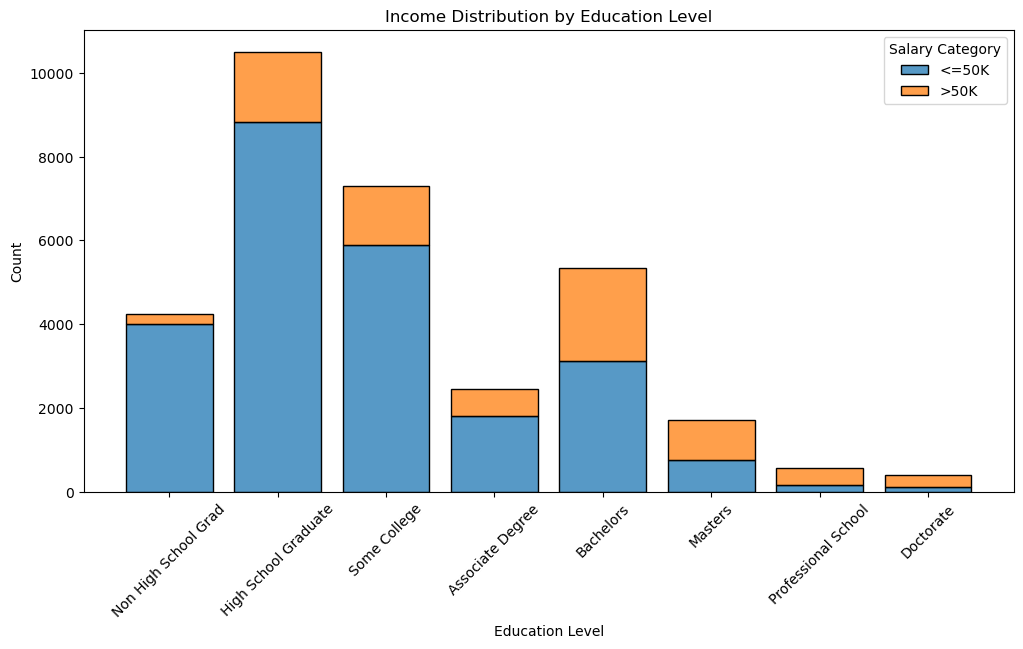
\includegraphics[width=1\linewidth]{hist_4.png}  % Reduce width slightly
    \caption{Final histogram for Income vs Education}
    \label{fig:final_income_vs_education}
\end{figure}
\section{Key Insights from Education Level vs. Income Distribution}

\begin{itemize}
    \item \textbf{Higher Education Correlates with Higher Income:} Individuals with advanced degrees (Masters, Professional School, Doctorate) have a significantly higher proportion of incomes above \$50K compared to those with lower educational attainment.
    
    \item \textbf{Most Common Education Levels:} The majority of individuals fall into the \textit{High School Graduate} and \textit{Some College} categories, making them the largest groups in the dataset. However, their income distributions do not show their education to be a predictor for the less than \$50K and greater than \$50K groups.
    
    \item \textbf{Education Alone is Not a Sole Predictor of Income:} Even at the Bachelor's level, a substantial number of individuals still earn less than \$50K. This suggests that additional factors such as work class, occupation, and experience must be considered to better predict income.
\end{itemize}


\section{User Stories}
To structure our approach further, we defined user stories that represent key stakeholders.

\underline{\textbf{User Story 1:}} 

The director of the UVW marketing team wants us to analyze how the
combination of sex, marital-status, and age influences salary category.

\textbf{Approach:} 

To combine the information for these groups, we broke apart ages into
categorical groups(bins), with a roughly gaussian distribution. The groups included:
17-20, 21-25, 26-32, 33-42, 43-54, 54-64, and 65+.

To compare age, marital status, and salary in one chart we chose to do a heatmap with a diverging color scheme of
'coolwarm' to represent low versus high percentages earning salaries $>$50K. Two facets were created, one representing male and the other female. 
Missing values were replaced with zeroes for this chart because in this case, we can take it to mean there was a lack
of participants who filled these categories. This helps clarify the visual representation of this data.

Another aspect that was considered was the center of the color scale. At the typical 0.5, coolwarm diverges into two solid colors.
Since many of the individual cells in the table are on the cool side and close to zero, the solid color becomes distracting.
The center of the scale was changed to 0.15 to give better differentiation for those percentages within the 10-40\% range.

Layout was also considered as a side-by-side was initially presented. This led to direct visual comparison between the two charts,
whereas the vertical alignment of 2 rows and 1 column better allows for viewing the charts individually.


\begin{figure}[h]
    \centering
    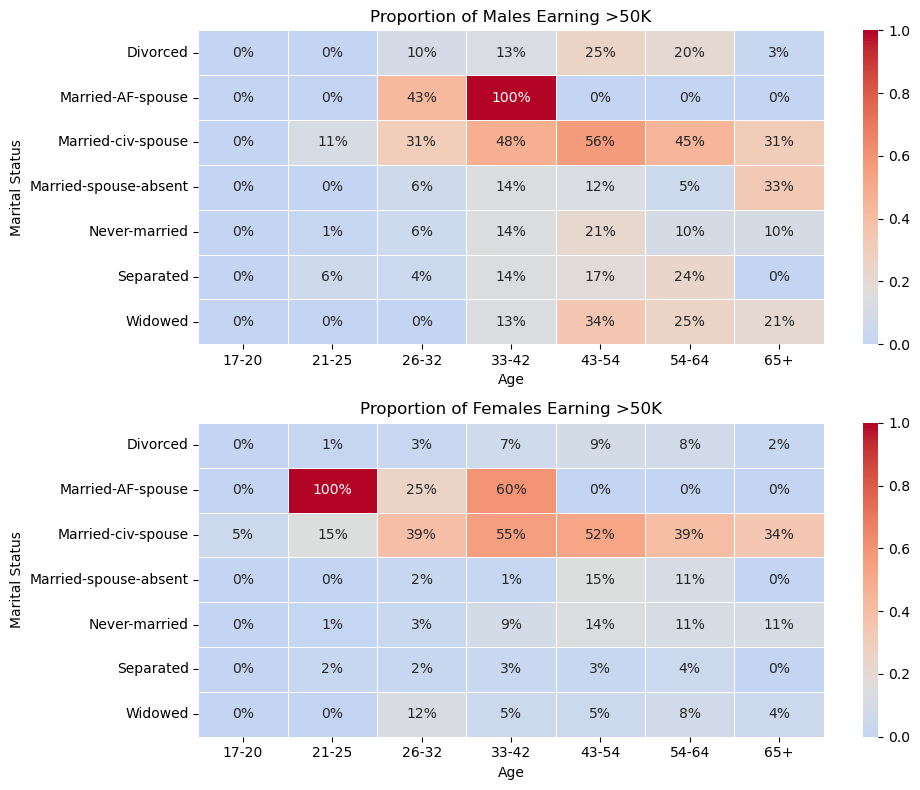
\includegraphics[width=1\linewidth]{mf_marital_agebins.png}  % Reduce width slightly
    \caption{Male and Female Salary by Marital Status vs Age}
    \label{fig:mf_marital_agebins}
\end{figure}


\textbf{Visual Analysis and Conclusions:} 
\medskip
    

For males, the highest-earning group falls within the 43-54 age range, with being
married by 25 serving as a strong indicator of future high salaries. This suggests
that marriage and middle age are strong correlates of higher income, potentially
due to greater career stability, shared financial resources, or long-term professional
growth. However, divorce or widowhood significantly reduces men’s earning potential,
indicating that life events can play a critical role in career trajectory.

For females, being married to a civilian spouse (Married-civ-spouse) is also a
strong predictor of high income, with earnings peaking in the 26-50 range (~54\%).
However, compared to men, married women are less likely to reach the highest income
brackets, reinforcing gender-based income disparities. Divorced, widowed, and
separated women show the weakest salary trends, with their earnings dropping
significantly. Married-spouse-absent and never-married women show slightly
higher earning potential (15\%) compared to the lowest-earning groups (3-9\%),
suggesting that some level of financial independence may mitigate these trends.

Overall, married individuals (Married-civ-spouse) of both genders are
the most likely to earn above 50K. Males in the 33-42 age range and
females in the 21-25 range who are Married-AF-spouse show an exceptionally
high proportion (1.0) of high earners, though this may be due to low sample sizes rather than a definitive trend.
\bigskip

\underline{\textbf{User Story 2:}}


A group of UVW Foreign relations researchers would like us to compare income variations among individuals based on their native country and work class.

\textbf{Approach:} 

When analyzing our dataset, we found that the number of people surveyed with `native-country' as United-States vastly overwhelms the rest of the data. 
Therefore, we did a probability analysis to see those earning 50K or more as a percentage of each country's population. The number of countries is also very high and
the tail of the dataset becomes very narrow, meaning that we don't have a ton of samples to look at from less common countries. 
We took the U.S. and the top 5 most common countries in the dataset outside of the U.S. and combined them into one graph. 
Since this is proportional to earning salary, we removed the `without-pay' and `never-worked' columns to reduce visual clutter.
Then, our hue became `workclass' to meet the requirements of the user story.
The 50\% threshold line (red dashed line) serves as a key benchmark to determine which groups are more likely to be high earners.

\begin{figure}[h]
    \centering
    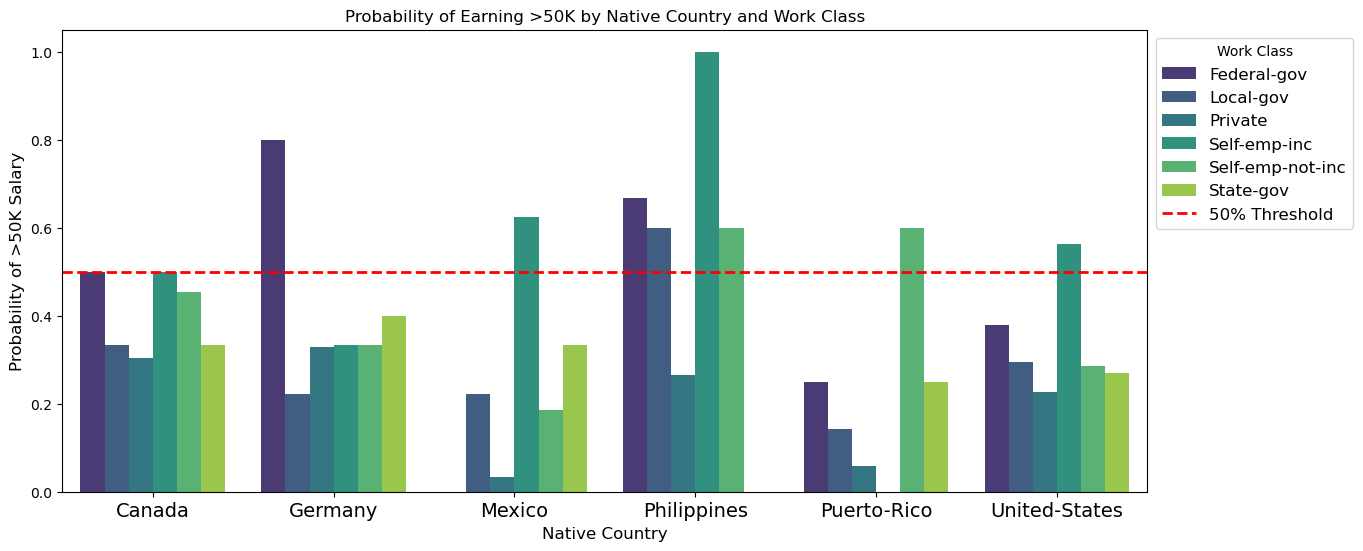
\includegraphics[width=1\linewidth]{country-workclass.png}  % Reduce width slightly
    \caption{Native Country - Workclass - Salary}
    \label{fig:mf_marital_agebins}
\end{figure}

\textbf{Visual Analysis and Conclusions:} 

\medskip

\underline{United States:}

\par A high proportion of self-emp-inc individuals surpass the 50\% threshold, making it one of the strongest predictors of high earnings.
Federal government jobs are the second highest, at nearly 40\%.

\underline{Germany:}

\par Germans who work in the federal government have are consistently high earners, with state government
employees the closest other category, while local government falls far behind.

\underline{Canada}

\par Canada has the most balanced distribution, with federal government and private workers both reaching the 50\% mark. 
Other groups fall behind, but they still maintain reasonable probabilities to earn high salaries.

\underline{Mexico:}

Mexico has a notable private sector that surpasses 50\%, while other positions show low probabilities for high salaries.

\underline{Puerto Rico:}

\par Puerto Rico exhibits the lowest earning probabilities overall, with many work classes failing to cross the 50\% threshold.
The exception seems to be the self-emp-not-inc category.

\underline{Philippines:}
\par The strongest self-employment signals come from the Philippines, where self-employed incorporated (self-emp-inc) individuals have the highest probability of earning $>$50K across all countries in this dataset.
Federal and state government jobs perform well, reaching around 50\%. Private-sector workers show more variance, with many remaining below the 50\% mark.

\medskip

The probability of earning $>$50K varies significantly across work
classes and countries, highlighting economic patterns that could
inform UVW College’s enrollment strategy. Across all countries,
self-employed incorporated (self-emp-inc) individuals consistently
rank among the highest earners, often surpassing the 50\% threshold.
Government jobs (federal-gov, state-gov, and local-gov) show moderate
earning probabilities (40-60\%), while private-sector employees
exhibit more country-dependent variation—with some nations reporting
strong earning potential and others remaining below the threshold.
Self-employed but not incorporated (self-emp-not-inc) workers exhibit
the widest earnings spread, indicating that their income levels fluctuate significantly based on country-specific factors.

Among individual countries, the Philippines stands out, with self-emp-inc
individuals having the highest probability of earning $>$50K across all nations.
In contrast, Puerto Rico exhibits the lowest earning probabilities overall,
with most work classes failing to exceed 50\%, except for self-emp-not-inc workers.
The United States, Canada, and Germany display more balanced distributions,
with federal government and self-emp-inc roles consistently ranking among
the highest earners. Mexico, however, stands out for its strong
private-sector performance, while Germany’s government employees (particularly at the federal level)
appear to have the most stable high-income probability.

\underline{\textbf{User Story 3:} }

Workforce development strategist is asking us to to 
compare income variations among individuals based on their sex and hours worked

\textbf{Approach:} 

We created a box plot for this analysis to compare 
income variations among individuals based on their sex and hours worked per week.
This visualization was chosen because it effectively displays distribution,
median work hours, interquartile range (IQR), and outliers, allowing us
to simply observe differences between $<$50K and $>$50K earners. The x-axis
represents hours worked per week, while the y-axis categorizes individuals by income group
in two region,with hue distinguishing between males and females.
The design process involved filtering relevant data and selecting a meaningful
color palette (blue for males and pink for females), and adjusting figure size
and median line thickness to enhance readability.

\begin{figure}[h]
    \centering
    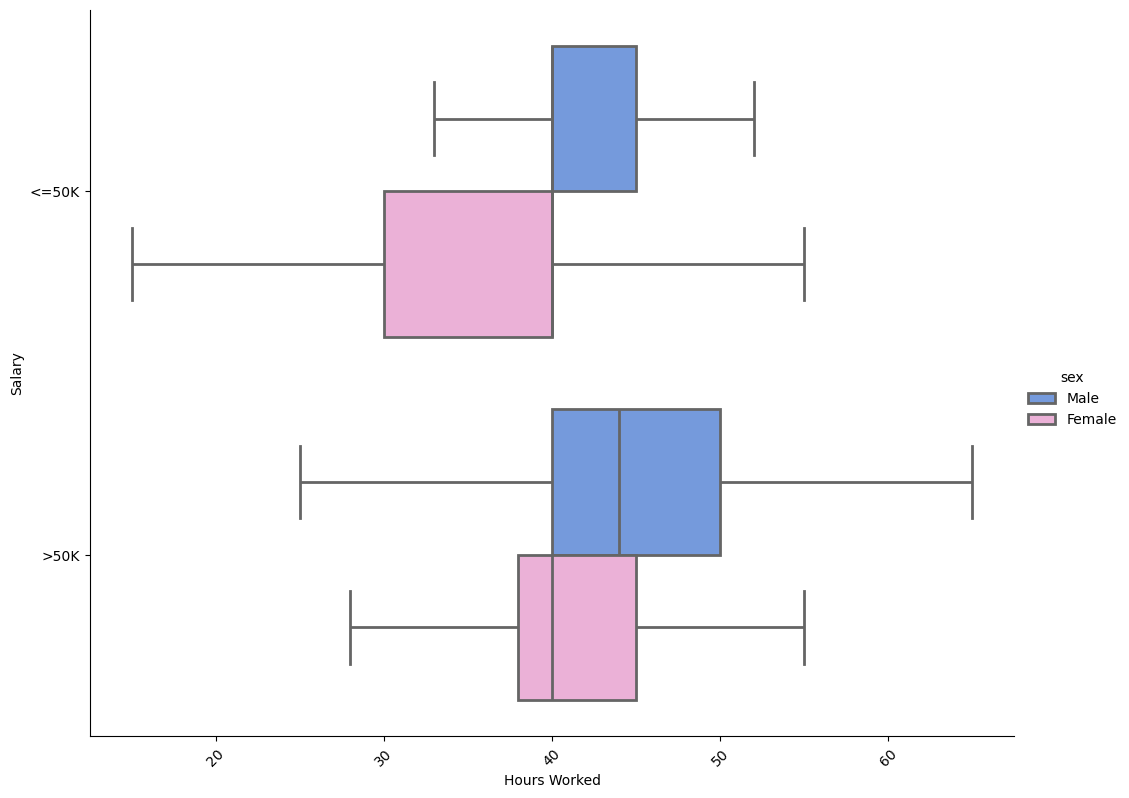
\includegraphics[width=1\linewidth]{gender_hours.png}  % Reduce width slightly
    \caption{Final histogram for Income vs Education}
    \label{fig:final_income_vs_education}
\end{figure}

\textbf{Visual Analysis and Conclusions:} 


Understanding how work hours vary by gender and salary level is crucial for UVW College’s
enrollment and marketing strategies. This analysis provides insight into which demographic
groups may be more likely to seek career advancement opportunities through higher education.

In both salary groups, males tend to work more hours per week than females,
with higher-income earners ($>$50K) working around 45 hours per week compared to
40 hours for lower-income earners ($<$50K). The variability in work hours is
significantly greater among those earning $>$50K, particularly for males,
suggesting that longer work schedules may contribute to higher salaries.
However, extreme workweeks ($>$60 hours per week) are more common in
high-earning males but rare among females. In contrast, the $<$50K group
has a much tighter work hour distribution (30-45 hours per week), with fewer outliers.

These findings indicate that longer work hours alone do not guarantee higher
pay, as factors such as occupation, education level, and industry play a
significant role in earnings potential. For UVW College, this suggests a
strategic opportunity to target professionals looking to upskill or transition
into higher-paying careers. Marketing efforts could emphasize degree programs
tailored to working professionals who want to increase earning potential without
requiring extreme work schedules. Additionally, understanding gender-based work
trends can help design flexible educational pathways that support
career growth for both men and women in different industries.

\smallskip

\underline{\textbf{User Story 4:}}

A group of UVW economic analysts wants us to examine how capital gains vary across different salary levels.

\textbf{Approach:} 

We created a histogram to analyze the distribution of capital-gain across
individuals earning $<$50K and more than 50K. This visualization was chosen because
capital gains are highly skewed, with most individuals reporting zero or
small values, while a few report very high values. To improve interpretability,
we filtered the data to exclude individuals with zero capital-gain and
those with gains exceeding \$15,000, which may be extreme outliers.
The histogram uses hue to differentiate between salary groups, allowing us to compare distributions directly.
The design process involved data filtering, selecting an
appropriate bin range(300 USD), and adjusting the color palette (blue for 50K plus, orange for $<$50K)
to enhance clarity and match previous charts. 

\begin{figure}[h]
    \centering
    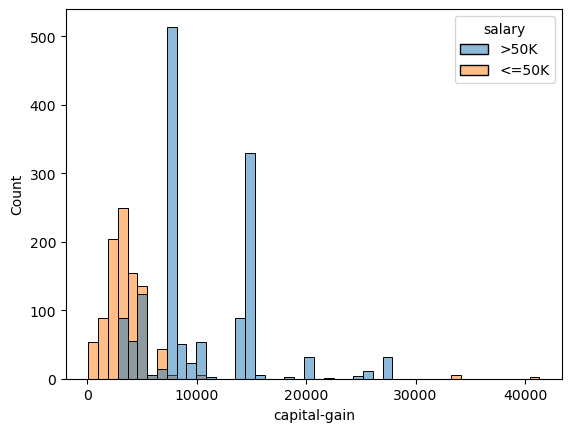
\includegraphics[width=1\linewidth]{capital-gain.png}  % Reduce width slightly
    \caption{Capital gain versus Salary}
    \label{fig:Capital gain - Salary}
\end{figure}

\textbf{Visual Analysis and Conclusions:} 

The plot reveals that high capital gains are disproportionately associated
with the high income group, whereas low earners rarely report significant
capital gains - a stark contrast between individuals earning above and below \$50K.
The histogram reveals that lower-income earners have a broader and
more continuous distribution of small capital gains, primarily
concentrated in the 0 to 5,000 range. In contrast, higher-income
earners show a range of higher level gains, with distinct peaks
around 8,000. This suggests that certain tax
incentives or capital gains brackets play a significant
role in wealth accumulation for high earners. The Kernel Density
Estimate (KDE) curves further reinforce this trend, with
lower-income individuals displaying a smoother distribution,
while high earners cluster around specific capital gain amounts. 

Notably, capital gains among lower-income earners are more variable,
while high earners tend to report standardized capital gain figures.
This could indicate structural factors such as stock options, executive bonuses,
or investment-related tax strategies that are prevalent among individuals earning more than \$50K.

The findings align with the overarching project goal of identifying key
socioeconomic factors influencing income levels. The strong correlation
between high capital gains and salaries above \$50K suggests that
investment income is a critical driver of financial success.
This insight is particularly relevant for **UVW College’s enrollment
and marketing strategies**, as it highlights the importance of
financial literacy and investment education in long-term wealth accumulation.
Programs tailored toward investment knowledge, stock market participation,
and financial planning could be valuable for prospective students aiming
for higher income brackets. Additionally, the stark divide in capital gains
between salary groups suggests that traditional wages alone may not be
sufficient for substantial wealth accumulation, reinforcing the need for
curriculum enhancements that address economic mobility through investments
and wealth-building strategies.

\medskip

\underline{\textbf{User Story 5:}}

A foreign relations researcher is interested in
understanding how capital gains vary based on relationship status
and whether this impacts income classification ($<$50K vs. $>$50K).
By analyzing this interaction, we aim to identify potential patterns
in wealth accumulation and financial benefits associated with different
relationship categories.

\textbf{Approach:} 

For this analysis, we used a point plot to examine the relationship between
capital gain, relationship type, and salary category. The x-axis represents
different relationship categories, while the y-axis displays capital gain.
The hue differentiates between lower earning individuals and those earning
more than 50K, allowing for a direct comparison. Capital gain is an important
financial metric as it reflects non-salary earnings such as stock sales,
dividends, or real estate profits. This visualization helps us determine
whether certain relationship groups tend to accumulate more capital gains
and how that correlates with their overall income classification.

The design process for this visualization involved choosing a point plot
because it effectively displays central tendencies and variability for
a continuous variable like capital gain across multiple categorical groups - 
relationship status and salary. The color scheme (blue for $<$50K, orange for more than 50K)
enhances clarity, and the error bars help us assess the spread and
reliability of the data in each category.

\begin{figure}[h]
    \centering
    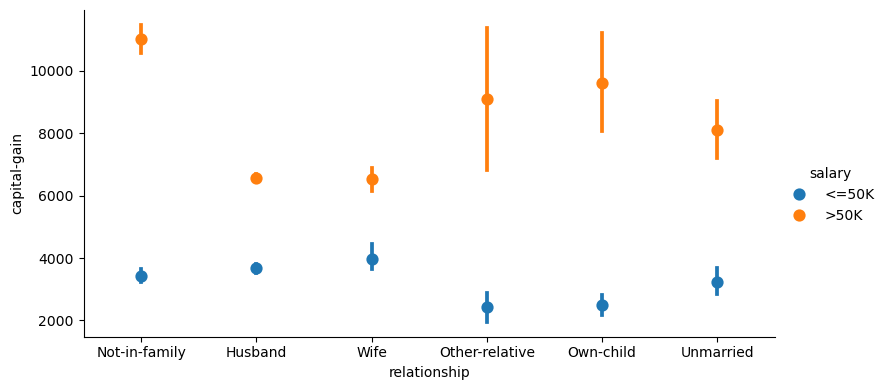
\includegraphics[width=1\linewidth]{capital-gain-relationship.png}  % Reduce width slightly
    \caption{Capital gain versus Relationship versus Salary}
    \label{fig:Capital gain - Relationship - Salary}
\end{figure}

\medskip
\textbf{Visual Analysis and Conclusions:} 

Across all relationship groups, individuals earning $>$50K report significantly
higher capital gains compared to those earning $<$50K. This reinforces that
investment income and financial assets are strong indicators of high-income status, beyond just salary.

Married individuals (husbands \& wives) exhibit moderate but stable capital
gains, which is expected since finances are often shared between spouses.
This suggests that financially stable married professionals may be
well-positioned for career advancement programs or executive education at UVW College.

Interestingly, “Other-relative” and “Own-child” categories in the $>$50K
group show exceptionally high capital gains ($8,000$+ USD) with large variance.
This suggests that some outlier cases—such as inheritance, trust funds, 
or investment-heavy individuals—exist within these groups. It also 
highlights that some financially independent adults earning a solid 
income still live within a larger household structure. These individuals
may be prime candidates for flexible, career-focused educational programs that fit their work-life balance.

Higher-income unmarried individuals report moderate capital gains ($6,000$–$8,000$ USD)
with high variation, indicating a mix of financial independence and investment activity.
In contrast, higher-income “Not-in-Family” individuals report extremely high capital gains ($10,000$+ USD),
potentially representing single professionals, older individuals with investment portfolios,
or those living with adult children while still working. This group could be a strong target
for professional certifications or advanced degrees aimed at career acceleration or entrepreneurship.

Lower-income individuals across these categories show capital gains in the $2,500$–$3,500$ USD
range, reinforcing the wealth gap between high and low earners. For UVW College,
this suggests a need for targeted financial aid, scholarships, and ROI-driven marketing
campaigns to ensure accessibility for lower-income learners while attracting financially
independent professionals to high-value programs.


\section{Key Questions and Solutions Implemented}

\par Throughout the project, several key questions emerged, requiring adjustments in \textbf{data processing, visualization techniques, and analysis methodology}. Below is a summary of these challenges and the solutions implemented to address them.

\subsection{Handling High-Variance Numerical Variables (Age \& Capital-Gain)}

\textbf{Problem:}  
Some variables, such as \textbf{age} and \textbf{capital-gain}, exhibited \textbf{high variance}, making it difficult to detect patterns using raw numerical values.  

\textbf{Solution Implemented:}  
\begin{itemize}
    \item Applied \textbf{domain-based binning} for age, grouping individuals into meaningful life stages (e.g., 18-25, 26-35, 36-45).  
    \item Used \textbf{data-driven binning} for capital-gain to reduce noise from extreme outliers while retaining critical distinctions.  
    \item Plotted \textbf{histograms} to validate bin selection and ensure the distribution remained meaningful.  
\end{itemize}

\subsection{Effective Visualization of Proportions in Categorical Variables}

\textbf{Problem:}  
Certain categorical variables, such as \textbf{relationship, occupation, and native-country}, contained many unique values, resulting in \textbf{cluttered bar charts}.  

\textbf{Solution Implemented:}  
\begin{itemize}
    \item Filtered and \textbf{only plotted the top 6 most frequent categories} to improve readability.  
    \item Used \textbf{stacked bar charts} and \textbf{mosaic plots} to compare proportions across different salary groups.  
    \item Implemented \textbf{hue differentiation} (\texttt{>50K} vs. \texttt{<50K}) to clearly distinguish high-income and low-income groups.  
\end{itemize}

\subsection{Managing Extreme Outliers in Capital-Gain}

\textbf{Problem:}  
The \textbf{capital-gain} variable was \textbf{highly skewed}, distorting visualizations and statistical summaries.  

\textbf{Solution Implemented:}  
\begin{itemize}
    \item \textbf{Filtered capital-gain values} below \textbf{\$15,000} to remove extreme cases while retaining meaningful variation.  
    \item \textbf{Applied log transformation} for exploratory analysis but ultimately \textbf{binned capital-gain values} for better interpretability.  
    \item \textbf{Compared before/after distributions} to ensure that trends were preserved.  
\end{itemize}

\subsection{Should Missing Values in the Heatmap Be Replaced?}

\textbf{Problem:}  
Some \textbf{age-bin and marital-status combinations} were missing values, resulting in \textbf{blank spaces in the heatmap}.  
This raised the question:  
\textit{Do these missing values mean there were no observations in the dataset, or that the probability is actually 0\%?}  

\textbf{Solution Implemented:}  
\begin{itemize}
    \item \textbf{Replaced missing values with 0\% instead of NaN (blank spaces)} based on the following considerations:  
    \begin{itemize}
        \item \textbf{Clarifies the Meaning of Missing Data}  
        - If a cell is missing, it likely means few people in that group earn \texttt{$>$50K}. 
        \item \textbf{Improves Visualization Consistency}  
        - Although the ideal would be to have a larger sample size, leaving NaNs creates \textbf{blank/white spaces}, making the heatmap look incomplete.  
        - Filling them with \textbf{0\% ensures all groups are visually represented}.  
    
    \end{itemize}
\end{itemize}


\section{Not Implemented / Planned Features}

\par Throughout the project, certain features were considered but ultimately not implemented,
while others were identified as potential future enhancements.

\begin{itemize}
    \item \textbf{Advanced Machine Learning Models for Income Prediction}  
    While classification models (Decision Trees, SVM, Neural Networks) were considered, the focus remained
    on exploratory data analysis and visualization of user stories rather than predictive modeling.  
    \textit{Reason for exclusion:} Scope limitations, and the primary goal of understanding trends rather than making predictions.

    \item \textbf{Additional Socioeconomic Data Integration}  
    External datasets (e.g., cost of living, inflation-adjusted wages) could have enriched the analysis, particularly for geographic trends.  
    \textit{Reason for exclusion:} Lack of easily accessible, well-structured external data within the project timeline.

    \item \textbf{Interactive Visualizations}  
    Future work could include interactive dashboards (e.g., Plotly, Tableau) that allow users to dynamically filter
    by attributes such as sex, workclass, and native country.

    \item \textbf{Expanded Time-Based Analysis}  
    The dataset represents a static snapshot, but tracking income trends over time (e.g., salary growth, career progression)
    would provide a more longitudinal perspective.

    \item \textbf{Predictive Modeling for Salary Estimation}  
    A logistic regression or decision tree model could be implemented to estimate the probability of earning $>$50K based on demographic and occupational factors.

    \item \textbf{Incorporation of Cost-of-Living Adjustments}  
    Salary alone does not reflect purchasing power—adjusting for regional cost-of-living differences would provide more accurate income comparisons.
\end{itemize}

\end{document}
